\documentclass[twoside]{book}

% Packages required by doxygen
\usepackage{fixltx2e}
\usepackage{calc}
\usepackage{doxygen}
\usepackage[export]{adjustbox} % also loads graphicx
\usepackage{graphicx}
\usepackage[utf8]{inputenc}
\usepackage{makeidx}
\usepackage{multicol}
\usepackage{multirow}
\PassOptionsToPackage{warn}{textcomp}
\usepackage{textcomp}
\usepackage[nointegrals]{wasysym}
\usepackage[table]{xcolor}

% Font selection
\usepackage[T1]{fontenc}
\usepackage[scaled=.90]{helvet}
\usepackage{courier}
\usepackage{amssymb}
\usepackage{sectsty}
\renewcommand{\familydefault}{\sfdefault}
\allsectionsfont{%
  \fontseries{bc}\selectfont%
  \color{darkgray}%
}
\renewcommand{\DoxyLabelFont}{%
  \fontseries{bc}\selectfont%
  \color{darkgray}%
}
\newcommand{\+}{\discretionary{\mbox{\scriptsize$\hookleftarrow$}}{}{}}

% Page & text layout
\usepackage{geometry}
\geometry{%
  a4paper,%
  top=2.5cm,%
  bottom=2.5cm,%
  left=2.5cm,%
  right=2.5cm%
}
\tolerance=750
\hfuzz=15pt
\hbadness=750
\setlength{\emergencystretch}{15pt}
\setlength{\parindent}{0cm}
\setlength{\parskip}{3ex plus 2ex minus 2ex}
\makeatletter
\renewcommand{\paragraph}{%
  \@startsection{paragraph}{4}{0ex}{-1.0ex}{1.0ex}{%
    \normalfont\normalsize\bfseries\SS@parafont%
  }%
}
\renewcommand{\subparagraph}{%
  \@startsection{subparagraph}{5}{0ex}{-1.0ex}{1.0ex}{%
    \normalfont\normalsize\bfseries\SS@subparafont%
  }%
}
\makeatother

% Headers & footers
\usepackage{fancyhdr}
\pagestyle{fancyplain}
\fancyhead[LE]{\fancyplain{}{\bfseries\thepage}}
\fancyhead[CE]{\fancyplain{}{}}
\fancyhead[RE]{\fancyplain{}{\bfseries\leftmark}}
\fancyhead[LO]{\fancyplain{}{\bfseries\rightmark}}
\fancyhead[CO]{\fancyplain{}{}}
\fancyhead[RO]{\fancyplain{}{\bfseries\thepage}}
\fancyfoot[LE]{\fancyplain{}{}}
\fancyfoot[CE]{\fancyplain{}{}}
\fancyfoot[RE]{\fancyplain{}{\bfseries\scriptsize Generated by Doxygen }}
\fancyfoot[LO]{\fancyplain{}{\bfseries\scriptsize Generated by Doxygen }}
\fancyfoot[CO]{\fancyplain{}{}}
\fancyfoot[RO]{\fancyplain{}{}}
\renewcommand{\footrulewidth}{0.4pt}
\renewcommand{\chaptermark}[1]{%
  \markboth{#1}{}%
}
\renewcommand{\sectionmark}[1]{%
  \markright{\thesection\ #1}%
}

% Indices & bibliography
\usepackage{natbib}
\usepackage[titles]{tocloft}
\setcounter{tocdepth}{3}
\setcounter{secnumdepth}{5}
\makeindex

% Hyperlinks (required, but should be loaded last)
\usepackage{ifpdf}
\ifpdf
  \usepackage[pdftex,pagebackref=true]{hyperref}
\else
  \usepackage[ps2pdf,pagebackref=true]{hyperref}
\fi
\hypersetup{%
  colorlinks=true,%
  linkcolor=blue,%
  citecolor=blue,%
  unicode%
}

% Custom commands
\newcommand{\clearemptydoublepage}{%
  \newpage{\pagestyle{empty}\cleardoublepage}%
}

\usepackage{caption}
\captionsetup{labelsep=space,justification=centering,font={bf},singlelinecheck=off,skip=4pt,position=top}

%===== C O N T E N T S =====

\begin{document}

% Titlepage & ToC
\hypersetup{pageanchor=false,
             bookmarksnumbered=true,
             pdfencoding=unicode
            }
\pagenumbering{alph}
\begin{titlepage}
\vspace*{7cm}
\begin{center}%
{\Large My Project }\\
\vspace*{1cm}
{\large Generated by Doxygen 1.8.12}\\
\end{center}
\end{titlepage}
\clearemptydoublepage
\pagenumbering{roman}
\tableofcontents
\clearemptydoublepage
\pagenumbering{arabic}
\hypersetup{pageanchor=true}

%--- Begin generated contents ---
\chapter{Hierarchical Index}
\section{Class Hierarchy}
This inheritance list is sorted roughly, but not completely, alphabetically\+:\begin{DoxyCompactList}
\item \contentsline{section}{Game\+Asset}{\pageref{classGameAsset}}{}
\begin{DoxyCompactList}
\item \contentsline{section}{Cube\+Asset}{\pageref{classCubeAsset}}{}
\item \contentsline{section}{Diamond\+Asset}{\pageref{classDiamondAsset}}{}
\end{DoxyCompactList}
\item \contentsline{section}{Game\+Asset\+Manager}{\pageref{classGameAssetManager}}{}
\item \contentsline{section}{Game\+World}{\pageref{classGameWorld}}{}
\item \contentsline{section}{Player}{\pageref{classPlayer}}{}
\item \contentsline{section}{S\+D\+L\+Window\+Deleter}{\pageref{structSDLWindowDeleter}}{}
\end{DoxyCompactList}

\chapter{Class Index}
\section{Class List}
Here are the classes, structs, unions and interfaces with brief descriptions\+:\begin{DoxyCompactList}
\item\contentsline{section}{\hyperlink{classCubeAsset}{Cube\+Asset} }{\pageref{classCubeAsset}}{}
\item\contentsline{section}{\hyperlink{classDiamondAsset}{Diamond\+Asset} }{\pageref{classDiamondAsset}}{}
\item\contentsline{section}{\hyperlink{classGameAsset}{Game\+Asset} }{\pageref{classGameAsset}}{}
\item\contentsline{section}{\hyperlink{classGameAssetManager}{Game\+Asset\+Manager} }{\pageref{classGameAssetManager}}{}
\item\contentsline{section}{\hyperlink{classGameWorld}{Game\+World} }{\pageref{classGameWorld}}{}
\item\contentsline{section}{\hyperlink{classPlayer}{Player} }{\pageref{classPlayer}}{}
\item\contentsline{section}{\hyperlink{structSDLWindowDeleter}{S\+D\+L\+Window\+Deleter} }{\pageref{structSDLWindowDeleter}}{}
\end{DoxyCompactList}

\chapter{Class Documentation}
\hypertarget{classCubeAsset}{}\section{Cube\+Asset Class Reference}
\label{classCubeAsset}\index{Cube\+Asset@{Cube\+Asset}}
Inheritance diagram for Cube\+Asset\+:\begin{figure}[H]
\begin{center}
\leavevmode
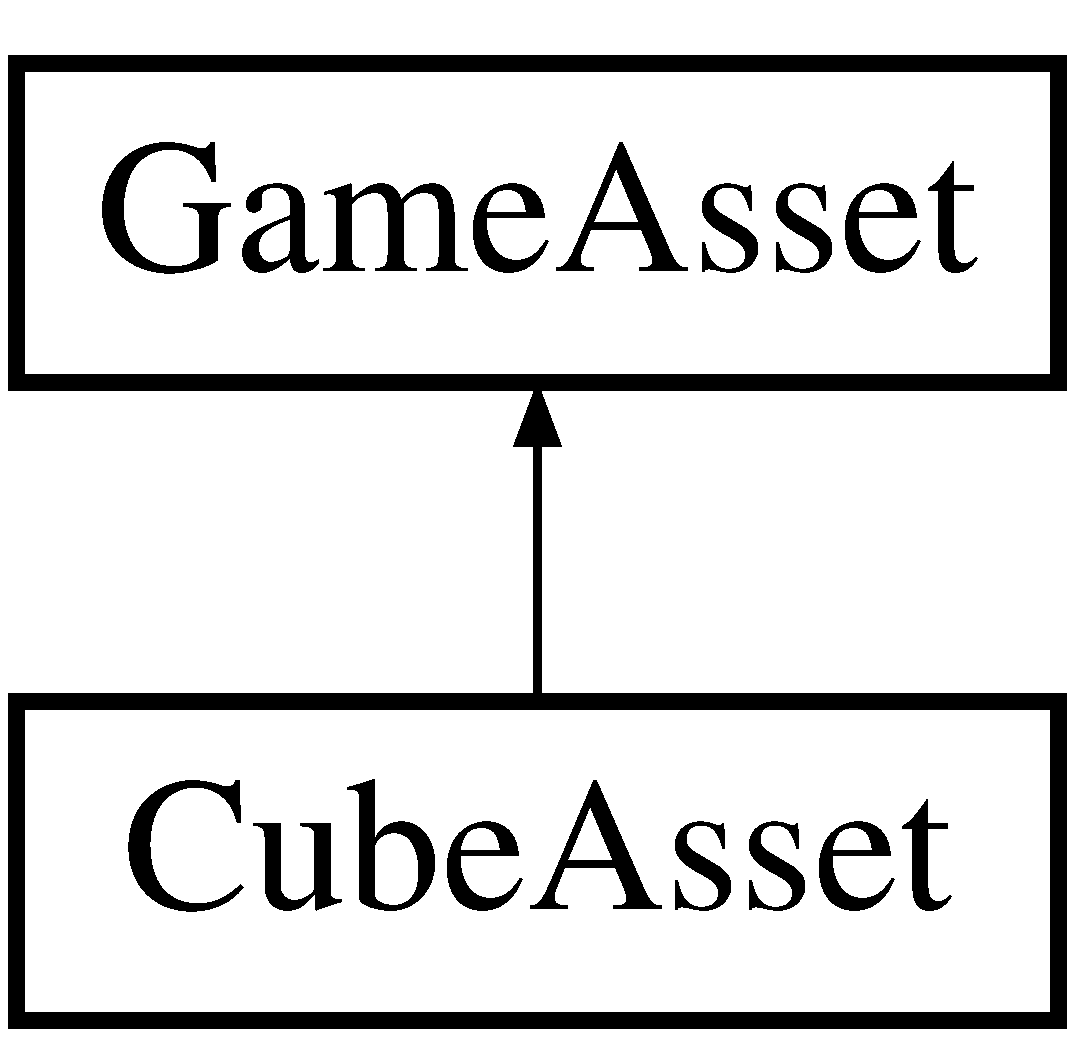
\includegraphics[height=2.000000cm]{classCubeAsset}
\end{center}
\end{figure}
\subsection*{Public Member Functions}
\begin{DoxyCompactItemize}
\item 
\hyperlink{classCubeAsset_a94f08a414e5b04ad37acffa3c1a1259b}{Cube\+Asset} (glm\+::vec3, glm\+::vec3)
\item 
virtual void {\bfseries Draw} (G\+Luint)\hypertarget{classCubeAsset_a1af568486056e254ffcf98fd99947bfe}{}\label{classCubeAsset_a1af568486056e254ffcf98fd99947bfe}

\end{DoxyCompactItemize}


\subsection{Constructor \& Destructor Documentation}
\index{Cube\+Asset@{Cube\+Asset}!Cube\+Asset@{Cube\+Asset}}
\index{Cube\+Asset@{Cube\+Asset}!Cube\+Asset@{Cube\+Asset}}
\subsubsection[{\texorpdfstring{Cube\+Asset(glm\+::vec3, glm\+::vec3)}{CubeAsset(glm::vec3, glm::vec3)}}]{\setlength{\rightskip}{0pt plus 5cm}Cube\+Asset\+::\+Cube\+Asset (
\begin{DoxyParamCaption}
\item[{glm\+::vec3}]{pos, }
\item[{glm\+::vec3}]{color}
\end{DoxyParamCaption}
)}\hypertarget{classCubeAsset_a94f08a414e5b04ad37acffa3c1a1259b}{}\label{classCubeAsset_a94f08a414e5b04ad37acffa3c1a1259b}
Initializes a new \hyperlink{classCubeAsset}{Cube\+Asset}. Passed in is a vec3 for the position and a vec3 for the colour values (R\+GB). 

The documentation for this class was generated from the following files\+:\begin{DoxyCompactItemize}
\item 
Cube\+Asset.\+h\item 
Cube\+Asset.\+cc\end{DoxyCompactItemize}

\hypertarget{classDiamondAsset}{}\section{Diamond\+Asset Class Reference}
\label{classDiamondAsset}\index{Diamond\+Asset@{Diamond\+Asset}}
Inheritance diagram for Diamond\+Asset\+:\begin{figure}[H]
\begin{center}
\leavevmode
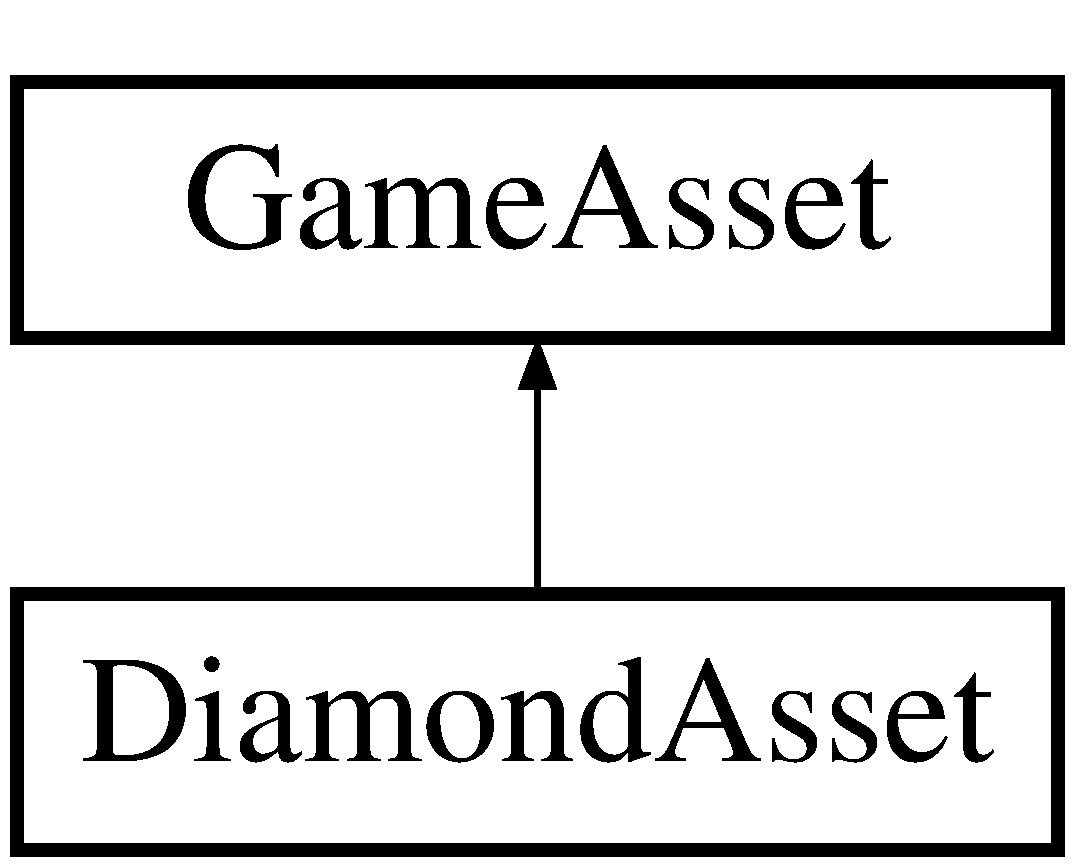
\includegraphics[height=2.000000cm]{classDiamondAsset}
\end{center}
\end{figure}
\subsection*{Public Member Functions}
\begin{DoxyCompactItemize}
\item 
\hyperlink{classDiamondAsset_af17cd961010d8b40199f8fe3b8dc1912}{Diamond\+Asset} (glm\+::vec3, glm\+::vec3)
\item 
virtual void {\bfseries Draw} (G\+Luint)\hypertarget{classDiamondAsset_a0c259031894623285b3b511321c73abb}{}\label{classDiamondAsset_a0c259031894623285b3b511321c73abb}

\end{DoxyCompactItemize}


\subsection{Constructor \& Destructor Documentation}
\index{Diamond\+Asset@{Diamond\+Asset}!Diamond\+Asset@{Diamond\+Asset}}
\index{Diamond\+Asset@{Diamond\+Asset}!Diamond\+Asset@{Diamond\+Asset}}
\subsubsection[{\texorpdfstring{Diamond\+Asset(glm\+::vec3, glm\+::vec3)}{DiamondAsset(glm::vec3, glm::vec3)}}]{\setlength{\rightskip}{0pt plus 5cm}Diamond\+Asset\+::\+Diamond\+Asset (
\begin{DoxyParamCaption}
\item[{glm\+::vec3}]{pos, }
\item[{glm\+::vec3}]{color}
\end{DoxyParamCaption}
)}\hypertarget{classDiamondAsset_af17cd961010d8b40199f8fe3b8dc1912}{}\label{classDiamondAsset_af17cd961010d8b40199f8fe3b8dc1912}
Initializes a new \hyperlink{classDiamondAsset}{Diamond\+Asset}. Passed in is a vec3 for the position and a vec3 for the colour values (R\+GB). 

The documentation for this class was generated from the following files\+:\begin{DoxyCompactItemize}
\item 
Diamond\+Asset.\+h\item 
Diamond\+Asset.\+cc\end{DoxyCompactItemize}

\hypertarget{classGameAsset}{}\section{Game\+Asset Class Reference}
\label{classGameAsset}\index{Game\+Asset@{Game\+Asset}}
Inheritance diagram for Game\+Asset\+:\begin{figure}[H]
\begin{center}
\leavevmode
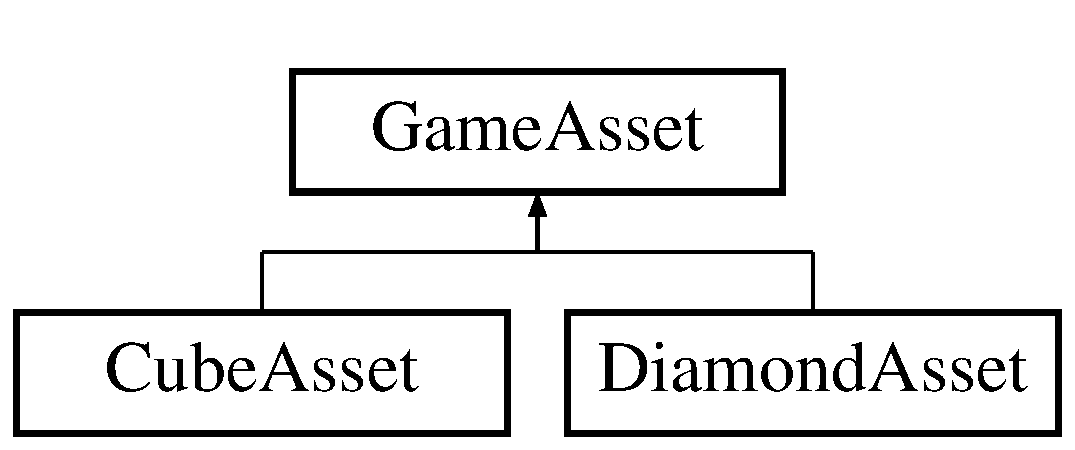
\includegraphics[height=2.000000cm]{classGameAsset}
\end{center}
\end{figure}
\subsection*{Public Member Functions}
\begin{DoxyCompactItemize}
\item 
virtual void {\bfseries Draw} (G\+Luint)=0\hypertarget{classGameAsset_a961aa51ca0a9961fc584c0b5d5431300}{}\label{classGameAsset_a961aa51ca0a9961fc584c0b5d5431300}

\end{DoxyCompactItemize}


The documentation for this class was generated from the following file\+:\begin{DoxyCompactItemize}
\item 
Game\+Asset.\+h\end{DoxyCompactItemize}

\hypertarget{classGameAssetManager}{}\section{Game\+Asset\+Manager Class Reference}
\label{classGameAssetManager}\index{Game\+Asset\+Manager@{Game\+Asset\+Manager}}


{\ttfamily \#include $<$Game\+Asset\+Manager.\+h$>$}

\subsection*{Public Member Functions}
\begin{DoxyCompactItemize}
\item 
\hyperlink{classGameAssetManager_aaa0d58e276cc10ad91a7457085598a71}{Game\+Asset\+Manager} (Application\+Mode)
\item 
virtual \hyperlink{classGameAssetManager_a1270bd61ecbcca563f079803e40c9b77}{$\sim$\+Game\+Asset\+Manager} ()
\item 
\hyperlink{classGameAssetManager_a2c9adcb72faa154c87eadc9bafe5269d}{Game\+Asset\+Manager} (\hyperlink{classGameAssetManager}{Game\+Asset\+Manager} const \&)
\item 
\hyperlink{classGameAssetManager_a44f6e2fd6b8ff1dd64e5697f1be7386d}{Game\+Asset\+Manager} (\hyperlink{classGameAssetManager}{Game\+Asset\+Manager} const \&\&)
\item 
void \hyperlink{classGameAssetManager_ac72678a4ad5378c685aa6bae84a4e712}{operator=} (\hyperlink{classGameAssetManager}{Game\+Asset\+Manager} const \&)
\item 
void \hyperlink{classGameAssetManager_ad3de8ff00d55ba04728b1de8213b2349}{Add\+Asset} (std\+::shared\+\_\+ptr$<$ \hyperlink{classGameAsset}{Game\+Asset} $>$)
\item 
void \hyperlink{classGameAssetManager_a32837132bd70a9a9ed537323c2d3d886}{Draw} ()
\item 
G\+Luint {\bfseries return\+\_\+token} ()\hypertarget{classGameAssetManager_ad9795f6c4fb62772fcb1a8bbf2f99fc4}{}\label{classGameAssetManager_ad9795f6c4fb62772fcb1a8bbf2f99fc4}

\end{DoxyCompactItemize}


\subsection{Detailed Description}
\hyperlink{classGameAssetManager}{Game\+Asset\+Manager} is a container for Game\+Assets. It also provides utility functions to to create a simple Open\+GL program that can be used to draw a simple \hyperlink{classGameAsset}{Game\+Asset}. 

\subsection{Constructor \& Destructor Documentation}
\index{Game\+Asset\+Manager@{Game\+Asset\+Manager}!Game\+Asset\+Manager@{Game\+Asset\+Manager}}
\index{Game\+Asset\+Manager@{Game\+Asset\+Manager}!Game\+Asset\+Manager@{Game\+Asset\+Manager}}
\subsubsection[{\texorpdfstring{Game\+Asset\+Manager(\+Application\+Mode)}{GameAssetManager(ApplicationMode)}}]{\setlength{\rightskip}{0pt plus 5cm}Game\+Asset\+Manager\+::\+Game\+Asset\+Manager (
\begin{DoxyParamCaption}
\item[{Application\+Mode}]{mode}
\end{DoxyParamCaption}
)\hspace{0.3cm}{\ttfamily [explicit]}}\hypertarget{classGameAssetManager_aaa0d58e276cc10ad91a7457085598a71}{}\label{classGameAssetManager_aaa0d58e276cc10ad91a7457085598a71}
Creates a \hyperlink{classGameAssetManager}{Game\+Asset\+Manager} to load the correct shaders based on the Application\+Mode. \index{Game\+Asset\+Manager@{Game\+Asset\+Manager}!````~Game\+Asset\+Manager@{$\sim$\+Game\+Asset\+Manager}}
\index{````~Game\+Asset\+Manager@{$\sim$\+Game\+Asset\+Manager}!Game\+Asset\+Manager@{Game\+Asset\+Manager}}
\subsubsection[{\texorpdfstring{$\sim$\+Game\+Asset\+Manager()}{~GameAssetManager()}}]{\setlength{\rightskip}{0pt plus 5cm}Game\+Asset\+Manager\+::$\sim$\+Game\+Asset\+Manager (
\begin{DoxyParamCaption}
{}
\end{DoxyParamCaption}
)\hspace{0.3cm}{\ttfamily [virtual]}}\hypertarget{classGameAssetManager_a1270bd61ecbcca563f079803e40c9b77}{}\label{classGameAssetManager_a1270bd61ecbcca563f079803e40c9b77}
Deletes a \hyperlink{classGameAssetManager}{Game\+Asset\+Manager}, in particular it will clean up any modifications to the Open\+GL state. \index{Game\+Asset\+Manager@{Game\+Asset\+Manager}!Game\+Asset\+Manager@{Game\+Asset\+Manager}}
\index{Game\+Asset\+Manager@{Game\+Asset\+Manager}!Game\+Asset\+Manager@{Game\+Asset\+Manager}}
\subsubsection[{\texorpdfstring{Game\+Asset\+Manager(\+Game\+Asset\+Manager const \&)}{GameAssetManager(GameAssetManager const &)}}]{\setlength{\rightskip}{0pt plus 5cm}Game\+Asset\+Manager\+::\+Game\+Asset\+Manager (
\begin{DoxyParamCaption}
\item[{{\bf Game\+Asset\+Manager} const \&}]{the\+\_\+manager}
\end{DoxyParamCaption}
)}\hypertarget{classGameAssetManager_a2c9adcb72faa154c87eadc9bafe5269d}{}\label{classGameAssetManager_a2c9adcb72faa154c87eadc9bafe5269d}
Unimplemented copy constructor -- this means that the \hyperlink{classGameAssetManager}{Game\+Asset\+Manager} may not work as you\textquotesingle{}d expect when being copied. \index{Game\+Asset\+Manager@{Game\+Asset\+Manager}!Game\+Asset\+Manager@{Game\+Asset\+Manager}}
\index{Game\+Asset\+Manager@{Game\+Asset\+Manager}!Game\+Asset\+Manager@{Game\+Asset\+Manager}}
\subsubsection[{\texorpdfstring{Game\+Asset\+Manager(\+Game\+Asset\+Manager const \&\&)}{GameAssetManager(GameAssetManager const &&)}}]{\setlength{\rightskip}{0pt plus 5cm}Game\+Asset\+Manager\+::\+Game\+Asset\+Manager (
\begin{DoxyParamCaption}
\item[{{\bf Game\+Asset\+Manager} const \&\&}]{the\+\_\+manager}
\end{DoxyParamCaption}
)}\hypertarget{classGameAssetManager_a44f6e2fd6b8ff1dd64e5697f1be7386d}{}\label{classGameAssetManager_a44f6e2fd6b8ff1dd64e5697f1be7386d}
Unimplemented move constructor -- this unimplemented method violates the C++11 move semantics for \hyperlink{classGameAssetManager}{Game\+Asset\+Manager}. 

\subsection{Member Function Documentation}
\index{Game\+Asset\+Manager@{Game\+Asset\+Manager}!Add\+Asset@{Add\+Asset}}
\index{Add\+Asset@{Add\+Asset}!Game\+Asset\+Manager@{Game\+Asset\+Manager}}
\subsubsection[{\texorpdfstring{Add\+Asset(std\+::shared\+\_\+ptr$<$ Game\+Asset $>$)}{AddAsset(std::shared_ptr< GameAsset >)}}]{\setlength{\rightskip}{0pt plus 5cm}void Game\+Asset\+Manager\+::\+Add\+Asset (
\begin{DoxyParamCaption}
\item[{std\+::shared\+\_\+ptr$<$ {\bf Game\+Asset} $>$}]{the\+\_\+asset}
\end{DoxyParamCaption}
)}\hypertarget{classGameAssetManager_ad3de8ff00d55ba04728b1de8213b2349}{}\label{classGameAssetManager_ad3de8ff00d55ba04728b1de8213b2349}
Adds a \hyperlink{classGameAsset}{Game\+Asset} to the scene graph. \index{Game\+Asset\+Manager@{Game\+Asset\+Manager}!Draw@{Draw}}
\index{Draw@{Draw}!Game\+Asset\+Manager@{Game\+Asset\+Manager}}
\subsubsection[{\texorpdfstring{Draw()}{Draw()}}]{\setlength{\rightskip}{0pt plus 5cm}void Game\+Asset\+Manager\+::\+Draw (
\begin{DoxyParamCaption}
{}
\end{DoxyParamCaption}
)}\hypertarget{classGameAssetManager_a32837132bd70a9a9ed537323c2d3d886}{}\label{classGameAssetManager_a32837132bd70a9a9ed537323c2d3d886}
Draws each \hyperlink{classGameAsset}{Game\+Asset} in the scene graph. \index{Game\+Asset\+Manager@{Game\+Asset\+Manager}!operator=@{operator=}}
\index{operator=@{operator=}!Game\+Asset\+Manager@{Game\+Asset\+Manager}}
\subsubsection[{\texorpdfstring{operator=(\+Game\+Asset\+Manager const \&)}{operator=(GameAssetManager const &)}}]{\setlength{\rightskip}{0pt plus 5cm}void Game\+Asset\+Manager\+::operator= (
\begin{DoxyParamCaption}
\item[{{\bf Game\+Asset\+Manager} const \&}]{the\+\_\+manager}
\end{DoxyParamCaption}
)}\hypertarget{classGameAssetManager_ac72678a4ad5378c685aa6bae84a4e712}{}\label{classGameAssetManager_ac72678a4ad5378c685aa6bae84a4e712}
Unimplemented assisgnment operator -- violates the expected semantics for assignment in C++11. 

The documentation for this class was generated from the following files\+:\begin{DoxyCompactItemize}
\item 
Game\+Asset\+Manager.\+h\item 
Game\+Asset\+Manager.\+cc\end{DoxyCompactItemize}

\hypertarget{classGameWorld}{}\section{Game\+World Class Reference}
\label{classGameWorld}\index{Game\+World@{Game\+World}}


{\ttfamily \#include $<$Game\+World.\+h$>$}

\subsection*{Public Member Functions}
\begin{DoxyCompactItemize}
\item 
\hyperlink{classGameWorld_a17a84e57a80600961088afc753036f89}{Game\+World} (Application\+Mode)
\item 
void \hyperlink{classGameWorld_a4e3d5cbb6241c8db5d7e74af509a02c1}{moveF} ()
\item 
void \hyperlink{classGameWorld_a1c5c6bd707c87d80573e558ab8ce018a}{moveB} ()
\item 
void \hyperlink{classGameWorld_af1728ec61cd2016030821261c8f79c34}{moveL} ()
\item 
void \hyperlink{classGameWorld_ab59dfdd281fac21eb6f2680711188598}{moveR} ()
\item 
void \hyperlink{classGameWorld_a219d46bb16bfb526bcf9b6957515d063}{moveU} ()
\item 
void \hyperlink{classGameWorld_a32b9c8230ef13f29e03f38b43e015ad9}{moveD} ()
\item 
void \hyperlink{classGameWorld_a71f6a1467ce47501dbcafd5a2cbfb1a2}{set\+Camera} (G\+Lfloat, G\+Lfloat)
\item 
void \hyperlink{classGameWorld_a275418607d8286979b276f165ad5876b}{Draw} ()
\item 
void \hyperlink{classGameWorld_abd2600f14a82010bfd39dc25a782fa59}{load\+Cubes\+From\+Image} (std\+::string)
\end{DoxyCompactItemize}


\subsection{Detailed Description}
\hyperlink{classGameWorld}{Game\+World} allows us to separate the management of the game world from the nuts and bolts of game loop initialisation. The \hyperlink{classGameWorld}{Game\+World} currently has a very simplified scene graph consisiting of a single \hyperlink{classGameAssetManager}{Game\+Asset\+Manager}. 

\subsection{Constructor \& Destructor Documentation}
\index{Game\+World@{Game\+World}!Game\+World@{Game\+World}}
\index{Game\+World@{Game\+World}!Game\+World@{Game\+World}}
\subsubsection[{\texorpdfstring{Game\+World(\+Application\+Mode)}{GameWorld(ApplicationMode)}}]{\setlength{\rightskip}{0pt plus 5cm}Game\+World\+::\+Game\+World (
\begin{DoxyParamCaption}
\item[{Application\+Mode}]{mode}
\end{DoxyParamCaption}
)}\hypertarget{classGameWorld_a17a84e57a80600961088afc753036f89}{}\label{classGameWorld_a17a84e57a80600961088afc753036f89}
We thread the Application\+Mode through the \hyperlink{classGameWorld}{Game\+World} ss we want to read it in from the user. Threading the state through the various function calls is preferable (in this case) to having some kind of global state. 

\subsection{Member Function Documentation}
\index{Game\+World@{Game\+World}!Draw@{Draw}}
\index{Draw@{Draw}!Game\+World@{Game\+World}}
\subsubsection[{\texorpdfstring{Draw()}{Draw()}}]{\setlength{\rightskip}{0pt plus 5cm}void Game\+World\+::\+Draw (
\begin{DoxyParamCaption}
{}
\end{DoxyParamCaption}
)}\hypertarget{classGameWorld_a275418607d8286979b276f165ad5876b}{}\label{classGameWorld_a275418607d8286979b276f165ad5876b}
Calling \hyperlink{classGameWorld_a275418607d8286979b276f165ad5876b}{Draw()} will draw the entire world. \index{Game\+World@{Game\+World}!load\+Cubes\+From\+Image@{load\+Cubes\+From\+Image}}
\index{load\+Cubes\+From\+Image@{load\+Cubes\+From\+Image}!Game\+World@{Game\+World}}
\subsubsection[{\texorpdfstring{load\+Cubes\+From\+Image(std\+::string)}{loadCubesFromImage(std::string)}}]{\setlength{\rightskip}{0pt plus 5cm}void Game\+World\+::load\+Cubes\+From\+Image (
\begin{DoxyParamCaption}
\item[{std\+::string}]{location}
\end{DoxyParamCaption}
)}\hypertarget{classGameWorld_abd2600f14a82010bfd39dc25a782fa59}{}\label{classGameWorld_abd2600f14a82010bfd39dc25a782fa59}
load\+Cubes\+From\+Image will load a plain ppm file, and use each pixels colour and position to place a cube in the \hyperlink{classGameWorld}{Game\+World}. Any pixels that are completly black (R\+GB 0,0,0) will be ignored as to allow the creation of something like a maze \index{Game\+World@{Game\+World}!moveB@{moveB}}
\index{moveB@{moveB}!Game\+World@{Game\+World}}
\subsubsection[{\texorpdfstring{move\+B()}{moveB()}}]{\setlength{\rightskip}{0pt plus 5cm}void Game\+World\+::moveB (
\begin{DoxyParamCaption}
{}
\end{DoxyParamCaption}
)}\hypertarget{classGameWorld_a1c5c6bd707c87d80573e558ab8ce018a}{}\label{classGameWorld_a1c5c6bd707c87d80573e558ab8ce018a}
moveB calls the \hyperlink{classPlayer}{Player} Class moveB function to allow the camera to \textquotesingle{}walk\textquotesingle{} backwards \index{Game\+World@{Game\+World}!moveD@{moveD}}
\index{moveD@{moveD}!Game\+World@{Game\+World}}
\subsubsection[{\texorpdfstring{move\+D()}{moveD()}}]{\setlength{\rightskip}{0pt plus 5cm}void Game\+World\+::moveD (
\begin{DoxyParamCaption}
{}
\end{DoxyParamCaption}
)}\hypertarget{classGameWorld_a32b9c8230ef13f29e03f38b43e015ad9}{}\label{classGameWorld_a32b9c8230ef13f29e03f38b43e015ad9}
moveD calls the \hyperlink{classPlayer}{Player} Class moveD function to allow the camera to \textquotesingle{}fly\textquotesingle{} downwards \index{Game\+World@{Game\+World}!moveF@{moveF}}
\index{moveF@{moveF}!Game\+World@{Game\+World}}
\subsubsection[{\texorpdfstring{move\+F()}{moveF()}}]{\setlength{\rightskip}{0pt plus 5cm}void Game\+World\+::moveF (
\begin{DoxyParamCaption}
{}
\end{DoxyParamCaption}
)}\hypertarget{classGameWorld_a4e3d5cbb6241c8db5d7e74af509a02c1}{}\label{classGameWorld_a4e3d5cbb6241c8db5d7e74af509a02c1}
moveF calls the \hyperlink{classPlayer}{Player} Class moveF function to allow the camera to \textquotesingle{}walk\textquotesingle{} forwards \index{Game\+World@{Game\+World}!moveL@{moveL}}
\index{moveL@{moveL}!Game\+World@{Game\+World}}
\subsubsection[{\texorpdfstring{move\+L()}{moveL()}}]{\setlength{\rightskip}{0pt plus 5cm}void Game\+World\+::moveL (
\begin{DoxyParamCaption}
{}
\end{DoxyParamCaption}
)}\hypertarget{classGameWorld_af1728ec61cd2016030821261c8f79c34}{}\label{classGameWorld_af1728ec61cd2016030821261c8f79c34}
moveL calls the \hyperlink{classPlayer}{Player} Class moveL function to allow the camera to \textquotesingle{}walk\textquotesingle{} to the left \index{Game\+World@{Game\+World}!moveR@{moveR}}
\index{moveR@{moveR}!Game\+World@{Game\+World}}
\subsubsection[{\texorpdfstring{move\+R()}{moveR()}}]{\setlength{\rightskip}{0pt plus 5cm}void Game\+World\+::moveR (
\begin{DoxyParamCaption}
{}
\end{DoxyParamCaption}
)}\hypertarget{classGameWorld_ab59dfdd281fac21eb6f2680711188598}{}\label{classGameWorld_ab59dfdd281fac21eb6f2680711188598}
moveR calls the \hyperlink{classPlayer}{Player} Class moveR function to allow the camera to \textquotesingle{}walk\textquotesingle{} to the right \index{Game\+World@{Game\+World}!moveU@{moveU}}
\index{moveU@{moveU}!Game\+World@{Game\+World}}
\subsubsection[{\texorpdfstring{move\+U()}{moveU()}}]{\setlength{\rightskip}{0pt plus 5cm}void Game\+World\+::moveU (
\begin{DoxyParamCaption}
{}
\end{DoxyParamCaption}
)}\hypertarget{classGameWorld_a219d46bb16bfb526bcf9b6957515d063}{}\label{classGameWorld_a219d46bb16bfb526bcf9b6957515d063}
moveU calls the \hyperlink{classPlayer}{Player} Class moveU function to allow the camera to \textquotesingle{}fly\textquotesingle{} upwards \index{Game\+World@{Game\+World}!set\+Camera@{set\+Camera}}
\index{set\+Camera@{set\+Camera}!Game\+World@{Game\+World}}
\subsubsection[{\texorpdfstring{set\+Camera(\+G\+Lfloat, G\+Lfloat)}{setCamera(GLfloat, GLfloat)}}]{\setlength{\rightskip}{0pt plus 5cm}void Game\+World\+::set\+Camera (
\begin{DoxyParamCaption}
\item[{G\+Lfloat}]{x, }
\item[{G\+Lfloat}]{y}
\end{DoxyParamCaption}
)}\hypertarget{classGameWorld_a71f6a1467ce47501dbcafd5a2cbfb1a2}{}\label{classGameWorld_a71f6a1467ce47501dbcafd5a2cbfb1a2}
set\+Camera calls the \hyperlink{classPlayer}{Player} Class set\+Camera function to adjust the camera view. Passed in are the x and y values that the camera has to move by 

The documentation for this class was generated from the following files\+:\begin{DoxyCompactItemize}
\item 
Game\+World.\+h\item 
Game\+World.\+cc\end{DoxyCompactItemize}

\hypertarget{classPlayer}{}\section{Player Class Reference}
\label{classPlayer}\index{Player@{Player}}


{\ttfamily \#include $<$Player.\+h$>$}

\subsection*{Public Member Functions}
\begin{DoxyCompactItemize}
\item 
{\bfseries Player} (G\+Luint)\hypertarget{classPlayer_a0f090add8ef5ced1841e7e3517e09c09}{}\label{classPlayer_a0f090add8ef5ced1841e7e3517e09c09}

\item 
void {\bfseries Draw} ()\hypertarget{classPlayer_a00ae3ebe88af8f9cfabd819176516a73}{}\label{classPlayer_a00ae3ebe88af8f9cfabd819176516a73}

\item 
void {\bfseries moveF} ()\hypertarget{classPlayer_a62dfb3a0d78231f2247aedbe28f2e4a6}{}\label{classPlayer_a62dfb3a0d78231f2247aedbe28f2e4a6}

\item 
void {\bfseries moveB} ()\hypertarget{classPlayer_a7f941c85236bbf5007f7cc4d584d8837}{}\label{classPlayer_a7f941c85236bbf5007f7cc4d584d8837}

\item 
void {\bfseries moveL} ()\hypertarget{classPlayer_a3cb72f5babfc5e06a02a06a99cda0d5e}{}\label{classPlayer_a3cb72f5babfc5e06a02a06a99cda0d5e}

\item 
void {\bfseries moveR} ()\hypertarget{classPlayer_aecdd233e935159c57e9adf69ac3c1e14}{}\label{classPlayer_aecdd233e935159c57e9adf69ac3c1e14}

\item 
void {\bfseries moveU} ()\hypertarget{classPlayer_a813cc9bf7d1fee3db6fa863ebbcac502}{}\label{classPlayer_a813cc9bf7d1fee3db6fa863ebbcac502}

\item 
void {\bfseries moveD} ()\hypertarget{classPlayer_a7c99fd3922f9f3af779d8611be236853}{}\label{classPlayer_a7c99fd3922f9f3af779d8611be236853}

\item 
void {\bfseries set\+Camera} (G\+Lfloat, G\+Lfloat)\hypertarget{classPlayer_a41bae651f90eb67a84f801e89c6e6072}{}\label{classPlayer_a41bae651f90eb67a84f801e89c6e6072}

\item 
glm\+::vec3 {\bfseries get\+Min} ()\hypertarget{classPlayer_aed6199ac6d37ec3795750b4058a7230b}{}\label{classPlayer_aed6199ac6d37ec3795750b4058a7230b}

\item 
glm\+::vec3 {\bfseries get\+Max} ()\hypertarget{classPlayer_ae3e6a1b495d4c086a3ea7e2f10421971}{}\label{classPlayer_ae3e6a1b495d4c086a3ea7e2f10421971}

\end{DoxyCompactItemize}


\subsection{Detailed Description}
The \hyperlink{classPlayer}{Player} class is used to handle all thing relating to the cameras/characters position and movement in the game. 

The documentation for this class was generated from the following files\+:\begin{DoxyCompactItemize}
\item 
Player.\+h\item 
Player.\+cc\end{DoxyCompactItemize}

\hypertarget{structSDLWindowDeleter}{}\section{S\+D\+L\+Window\+Deleter Struct Reference}
\label{structSDLWindowDeleter}\index{S\+D\+L\+Window\+Deleter@{S\+D\+L\+Window\+Deleter}}
\subsection*{Public Member Functions}
\begin{DoxyCompactItemize}
\item 
void {\bfseries operator()} (S\+D\+L\+\_\+\+Window $\ast$window)\hypertarget{structSDLWindowDeleter_a2aedcc99c3756ae090c38badabeb10b1}{}\label{structSDLWindowDeleter_a2aedcc99c3756ae090c38badabeb10b1}

\end{DoxyCompactItemize}


The documentation for this struct was generated from the following file\+:\begin{DoxyCompactItemize}
\item 
main.\+cc\end{DoxyCompactItemize}

%--- End generated contents ---

% Index
\backmatter
\newpage
\phantomsection
\clearemptydoublepage
\addcontentsline{toc}{chapter}{Index}
\printindex

\end{document}
